\section{Design}
\label{Design}
When modelling penatgo in GROOVE, a board (start) graphtogether with transformations which model the game rules need to be defined.
Also a control program should be defined which defines the game flow.
It is preferred to keep the sub-board and player count scalable, so this requirement also needs to be taken into account.
There are multiple ways to model pentago, and in this section we will discuss our considerations and modelling choices when coming up with solutions.
The characteristics of GROOVE should be taken into account to optimize the simulation performance.

\subsection{Board Design}
The pentago board can be defined in multiple ways.
A trade-off has to be made between performance and scalability.

\subsubsection{Design 1}
\label{des1-board-design}

\begin{figure}[!h]
    \centering
    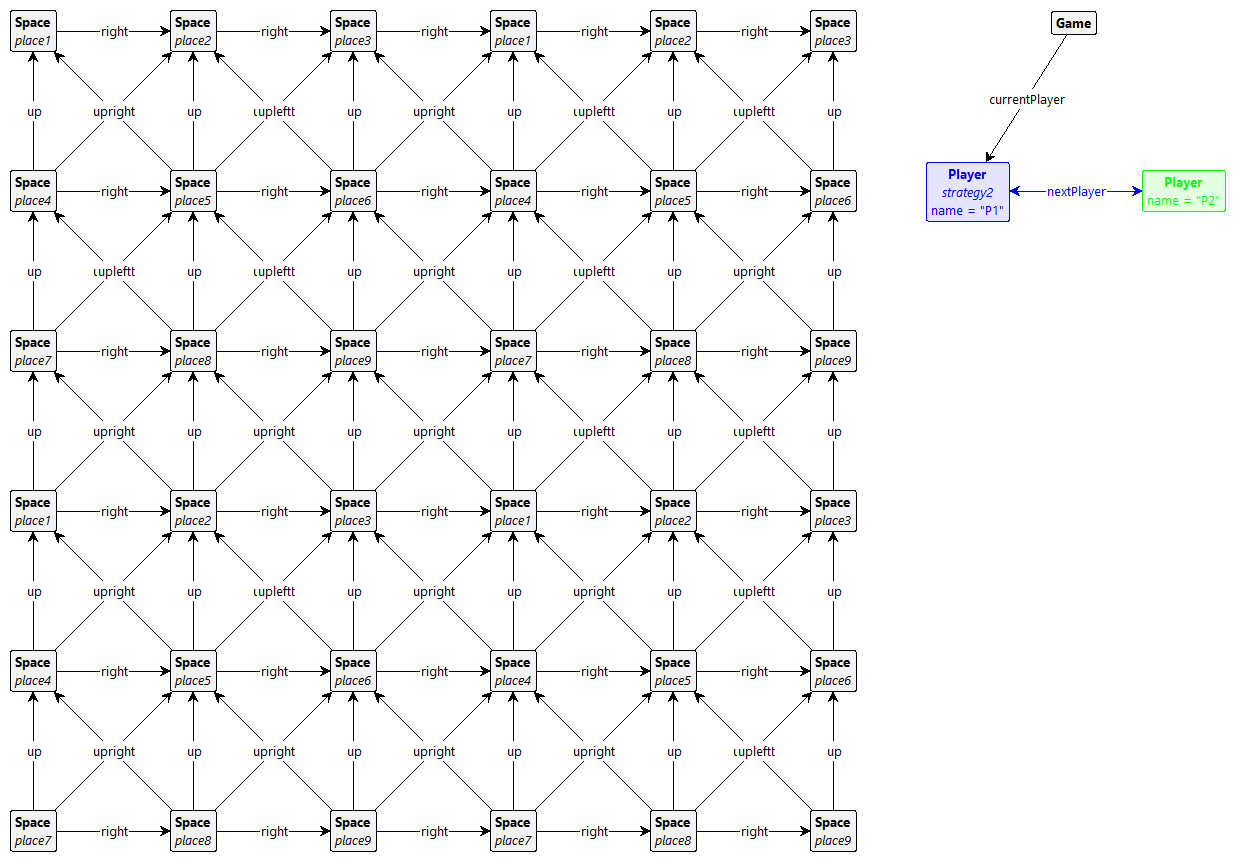
\includegraphics[scale=0.25,clip]{Images/board1.png}
    \caption{Design 1 board}
    \label{fig:board1}
\end{figure}

The default board contains 36 spaces, and two players.
Our first design features 36 spaces which are connected by horizontal, vertical and diagonal edges.
All spaces in a sub-board hold an unique identifier flag.
A game node and two players exist, where the game node maintains an edge to the player whoms turn it is.
The board model is displayed in figure \ref{fig:board1}.
A marble placement of a player on a space is defined as a edge from the player node to the space node.

\subsection{Rotating}
When a player has placed a marble, he has to rotate a sub-board.
This rotation can be seen as a graph transformation.
In this graph transformation the marbles on the sub-board are relocated to a position clockwise or counter-clockwise.

\subsubsection{Design 1}
\begin{figure}[!h]
    \centering
    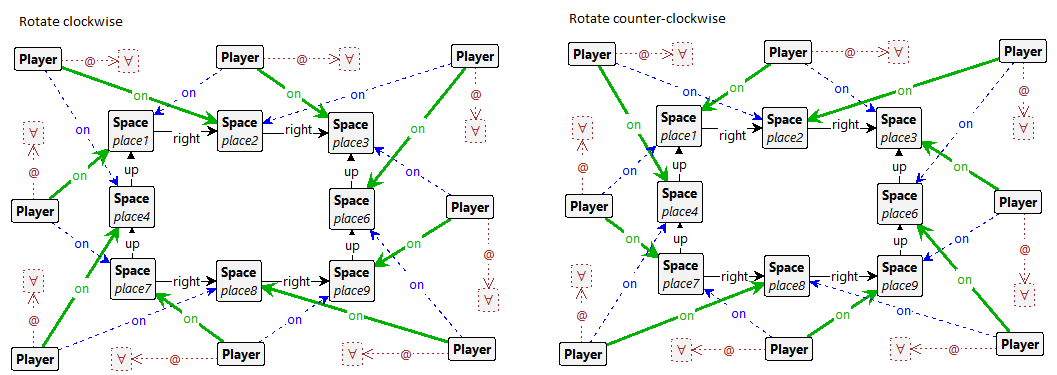
\includegraphics[scale=0.5,clip]{Images/rotate1.png}
    \caption{Design 1 rotations}
    \label{fig:rotate1}
\end{figure}

Because the nodes are fixed in the board defined in section \ref{des1-board-design}, we have chosen to only move the marbles instead of the whole sub-board.
This improves the complexity of this transformation but also that of the end-game detection, because board changes do not have to be taken into account.
Two transformations have been defined: one for the clockwise rotation and one for the counter-clockwise rotation.
Both transformations rotate all marbles on a sub-board 3 spaces in the respective direction.
The graph transformations defined for the rotations are displayed in figure \ref{fig:rotate1}.

\subsection{Taking turns}
In pentago, turns are taken between players. 
After a player has placed a marble, and rotated a sub-board, the other player gets a turn.
\subsubsection{Design 1}
\begin{figure}[!h]
    \centering
    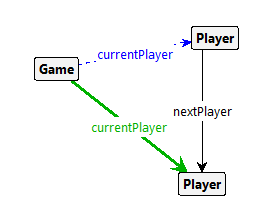
\includegraphics[scale=0.5,clip]{Images/turn1.png}
    \caption{Design 1 taking turns}
    \label{fig:turn1}
\end{figure}

The turn taking mechanism has been defined as a graph transformation.
In the start graph the participating players are defined with each player holding a nextPlayer edge to the player whoms turn it is after he is finished.
When a player has finished its turn, the currentPlayer edge from the game node is shifted to the player which is connected to by the nextPlayer edge.
The graph transformation defined for the turn taking is displayed in figure \ref{fig:turn1}.

\subsection{Checking for victory}
The game has ended when one player holds a row of 5 horizontal/vertical/diagonal consecutive nodes.
When no marbles can be placed on the board anymore the game results in a draw.

\subsubsection{Design 1}
\begin{figure}[!h]
    \centering
    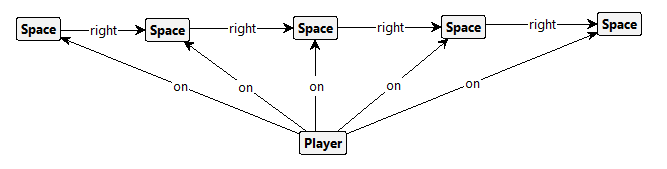
\includegraphics[scale=0.5,clip]{Images/endgame1.png}
    \caption{Design 1 victory checking}
    \label{fig:endgame1}
\end{figure}

The check for a winner condition has been modelled as a graph condition.
One player holds edges to five nodes which must be connected by either horizontal, vertical or diagonal edges.
The graph condition for a horizontal row is defined in figure \ref{fig:endgame1}.
The graph conditions which check for vertical or diagonal rows are identical, but they check for different node names.
A game is a draw when no placeMarble rules can be executed anymore.

\subsection{Design choices \& considerations not discussed so far}
To enforce that the game is played by the rules, a control program has been defined which holds the game flow.
As long as possible, a player places a marble, rotates a sub-board and gives the turn to the next player.
The game is finished when a win condition is met, or no marbles can be placed anymore.